\documentclass[a4paper,12pt]{exam}
\usepackage[utf8]{inputenc}
\usepackage[brazil]{babel}
\usepackage{amsmath}
\usepackage{amsfonts}
\usepackage{amssymb}
\usepackage{enumitem}
\usepackage{pdfpages}
\usepackage[margin=1.2in]{geometry}

% Informações da prova
\title{\vspace{-2.5cm} Prova Final}
%\date{\today}
\author{BCC740 - Inteligência Artificial}

% Customização do cabeçalho e rodapé
\pagestyle{headandfoot}
\firstpageheader{\textbf{BCC740 - Inteligência Artificial}}{}{\textbf{Data: \today}}
\runningheader{\textbf{BCC740 - Inteligência Artificial}}{}{Página \thepage\ de \numpages}
\firstpagefooter{}{}{}
\runningfooter{}{}{}

% Número de pontos e instruções
\pointsinrightmargin
\marginpointname{ -1 pt}
\pointformat{\bfseries}

% Configuração das perguntas
\setlength\linefillheight{.25in}

\begin{document}



\maketitle

\begin{enumerate}

    \item Quais são os critérios que definimos para medir a Inteligência de uma gente?

    \item Defina o problema de busca em espaços de estados. Apresente os seus componentes e o objetivo do problema.
    
    \item Qual(is) do(s) algoritmo(s) de busca a seguir apresenta(m) custo de \textbf{tempo} exponencial:
    \begin{enumerate}
        \item Busca em largura
        \item Busca em profundidade
        \item A$^*$
        \item Branch and Bound
    \end{enumerate}

    \item Qual(is) do(s) algoritmo(s) de busca a seguir apresenta(m) custo de \textbf{memória} exponencial:
    \begin{enumerate}
        \item Busca em largura
        \item Busca em profundidade
        \item A$^*$
        \item Branch and Bound
    \end{enumerate}

    \item Qual dos algoritmos a seguir remove da fronteira o caminho como o menor valor da soma entre o custo do caminho e a heurística?
    \begin{enumerate}
        \item Busca em largura
        \item Busca em profundidade
        \item A$^*$
        \item Branch and Bound
    \end{enumerate}

    \item O que é uma heurística admissível?

    \item Defina o problema de satisfação de restrições. Apresente os componentes e o objetivo do problema.
    
    \item Qual o objetivo do algoritmo GAC (Graph Arc Consistency)? 

    \item Resolva numericamente a rede neural abaixo:
    \clearpage
    \begin{figure}[!hb]
        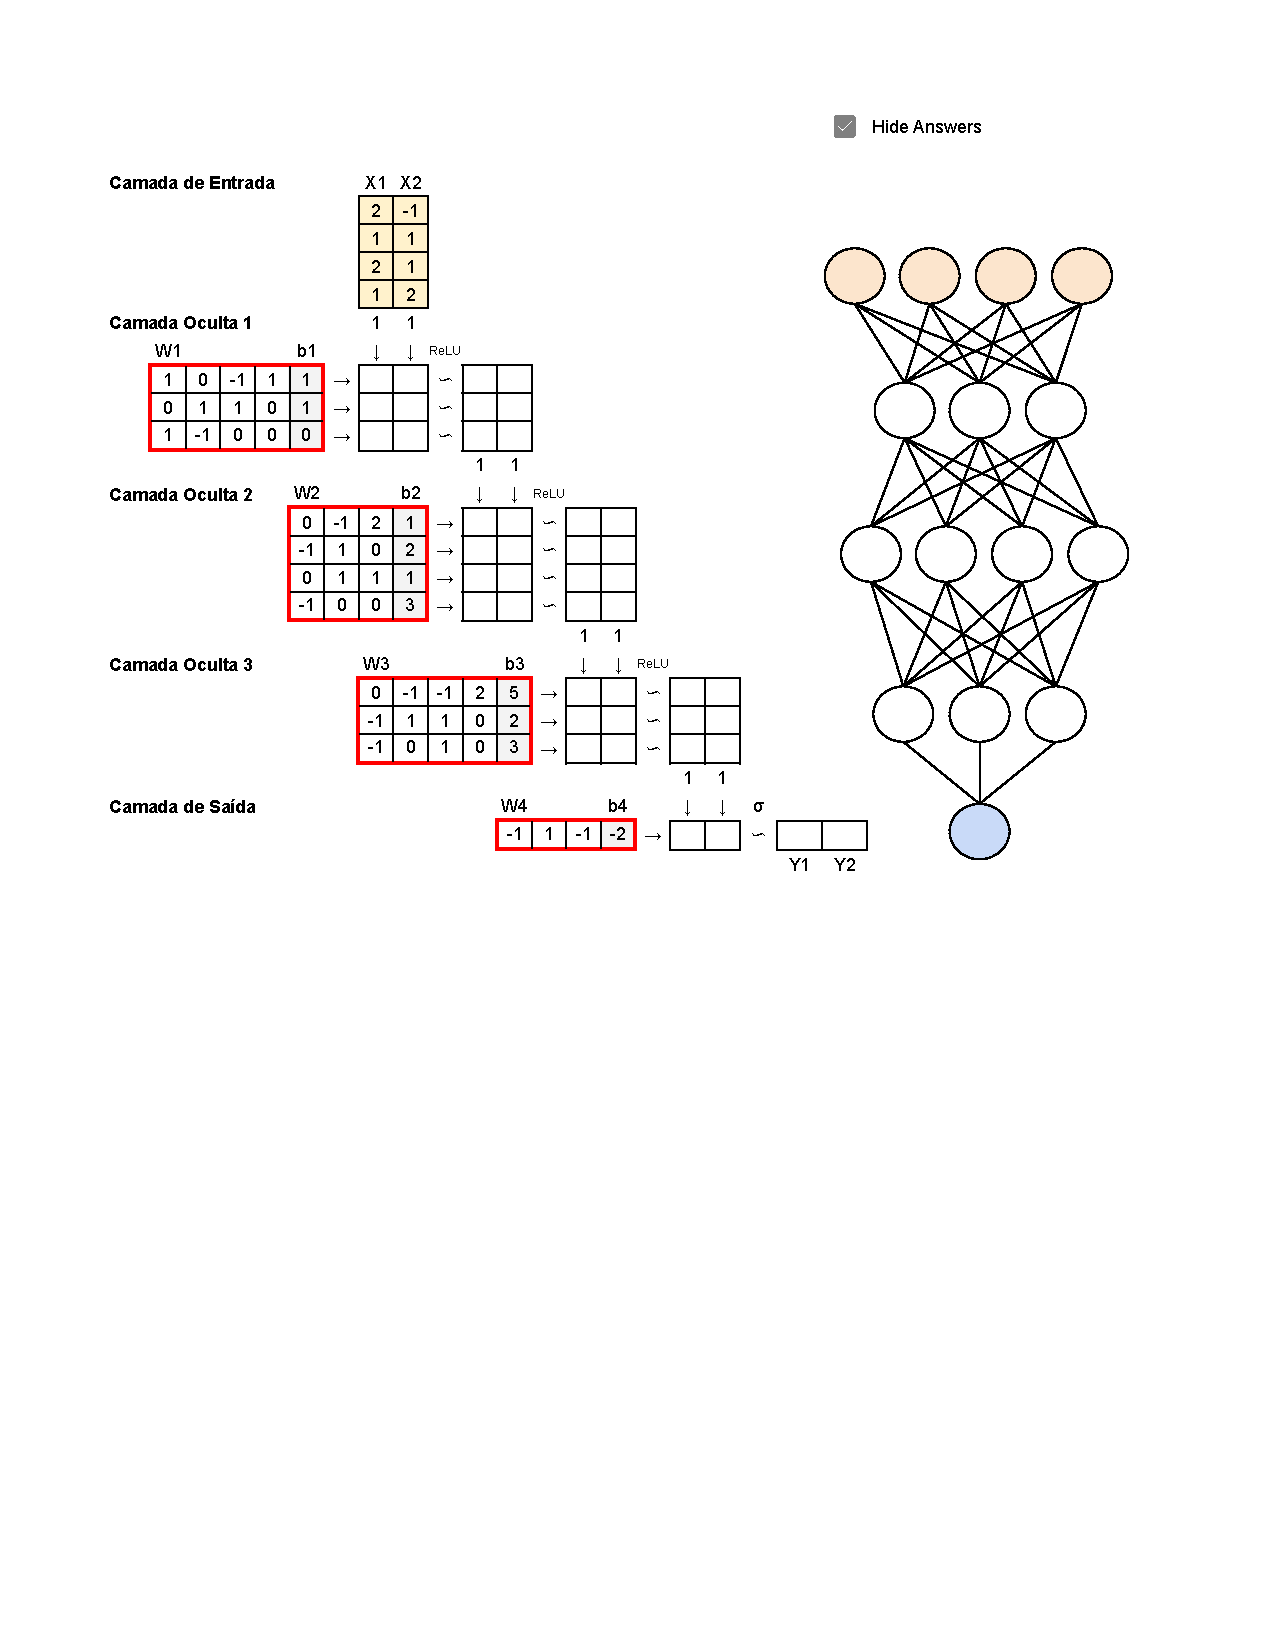
\includepdf[pages=-, trim=0cm 8cm 0cm 1cm, clip]{neural_network.pdf}
    \end{figure}
    \clearpage

    \item Considere um problema de \textbf{classificação}. Para os modelos abaixo responda: i) Qual é a arquitetura do modelo? ii) Qual a função de perda? iii) Qual o algoritmo de treinamento? 
        \begin{enumerate}
            \item Regressão Logística
            \item Árvore de decisão
            \item Rede Neural Artificial
        \end{enumerate}

    \item Considere um problema de \textbf{regressão}. Para os modelos abaixo responda: i) Qual é a arquitetura do modelo? ii) Qual a função de perda? iii) Qual o algoritmo de treinamento? 
    \begin{enumerate}
        \item Regressão Linear 
        \item Árvore de decisão
        \item Rede Neural Artificial
    \end{enumerate}

    \item Um modelo de regressão logística só consegue resolver tarefas de classificação quando as classes são linearmente separáveis. O que significa dizer que duas classes são linearmente separáveis? 

    \item Como uma rede neural resolve um problema de classificação no qual as classes não são linearmente separáveis, mesmo colocando uma sigmoid como função de ativação da saída?

    \item No artigo em que Alan Turing descreve o seu jogo da imitação, ele parece indicar que o entrevistado humano deveria ser uma mulher. Apresente argumentos para esta escolha.

\end{enumerate}

\end{document}
